%=====================================================================
\section{The wall lattice in ovals and ellipses}\label{sec:slattice}
Same analysis as Sec.~\ref{sec:clattice}, with positions measured by arclength along the real wall (Secs.~\ref{sec:md-fourier-static},
\ref{sec:md-fourier-dyn}, \ref{sec:md-drift}); 81 active oval and ellipse runs plus a $k=6$ circle reference run with the same script.
\begin{table}[H]\centering\small
\caption{Static wall Fourier, $k=6$ ($m_\mathrm{lat}=2k-2=10$). $S(m^*)$: peak of the instantaneous structure factor (a perfect
10-defect lattice gives $\approx10$); $f_\mathrm{static}$: 1 = pinned. Ranges over seeds.}\label{tab:sfourier}
\begin{adjustbox}{max width=\textwidth}
\begin{tabular}{lcccccc}\toprule
cavity & aspect & $N_\mathrm{wall}$ & $m^*$ & $S(m^*)$ & $f_\mathrm{static}$ & $\tau_\mathrm{fl}$\\\midrule
circles 1.43, $2.15\,\la$ & 1 & $\approx10$ & 10 & 9.0 & 0.99 & --\\
oval H48 $b/a=2.5$ & 1.18 & 8.6--8.8 & 10 & 7.1--7.3 & 0.97 & 12--18\\
oval H48 $b/a=2.0$ & 1.29 & 5.8--6.1 & 10 & 3.0--3.9 & 0.81--0.88 & 14--16\\
oval H48 $b/a=1.6$ & 1.51 & 5.6--6.1 & 9--10 & 1.7--2.7 & 0.15--0.67 & 80--308\\
oval H48 $b/a=1.3$ & 1.94 & 5.8--6.1 & 8--9 & 1.5--2.1 & 0.00--0.15 & 50--978\\
ellipse $\varepsilon=1.2$ & 1.2 & 9.8 & 10 & 8.0 & 0.98 & 10--14\\
ellipse $\varepsilon=1.5$ & 1.5 & 7.7 & 10 & 2.2--2.4 & 0.33--0.38 & 208--416\\
ellipse $\varepsilon=2.0$ & 2.0 & 7.3 & 8 & 1.4--1.8 & 0.06--0.15 & 138--142\\\bottomrule
\end{tabular}
\end{adjustbox}
\end{table}
\begin{figure}[H]\centering
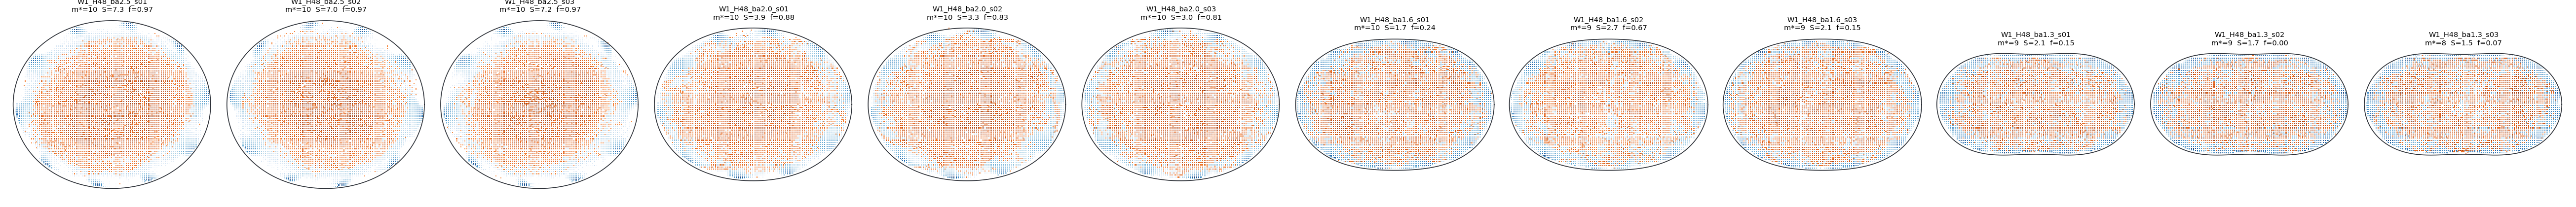
\includegraphics[width=\textwidth]{wf_maps_size.png}\\[4pt]
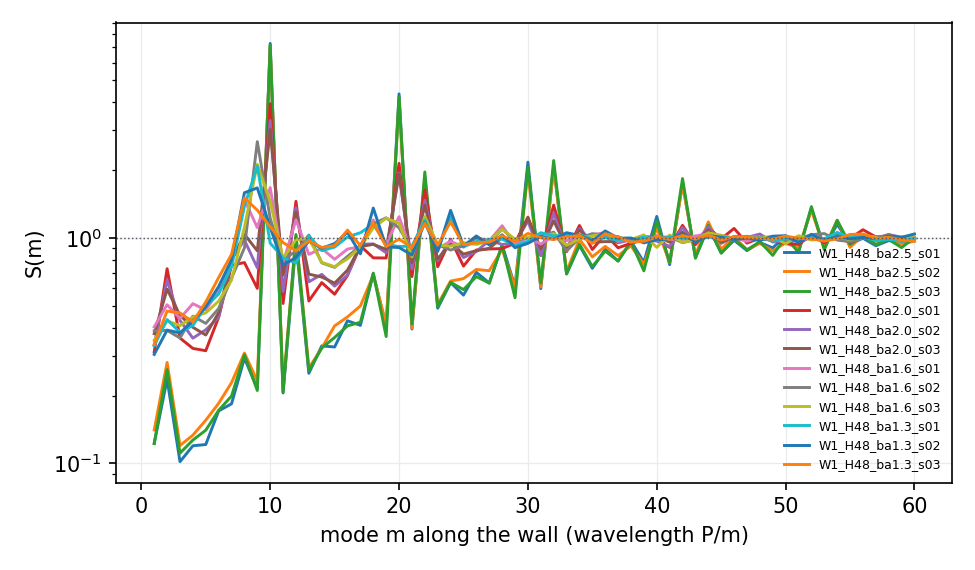
\includegraphics[width=0.7\textwidth]{wf_S_size.png}
\caption{Ovals of half-length $2.16\,\la$ (3 seeds): defect density maps with $m^*$, $S$ and $f_\mathrm{static}$ (top) and the structure
factor $S(m)$ along the wall (bottom).}\label{fig:wfsize}
\end{figure}
\begin{figure}[H]\centering
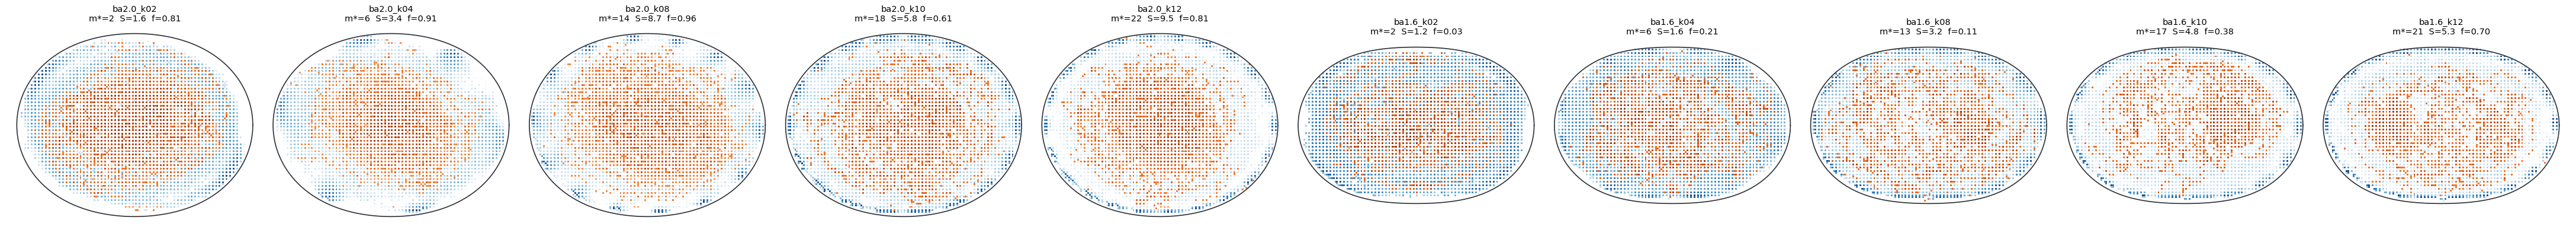
\includegraphics[width=\textwidth]{wf_maps_kscan.png}\\[4pt]
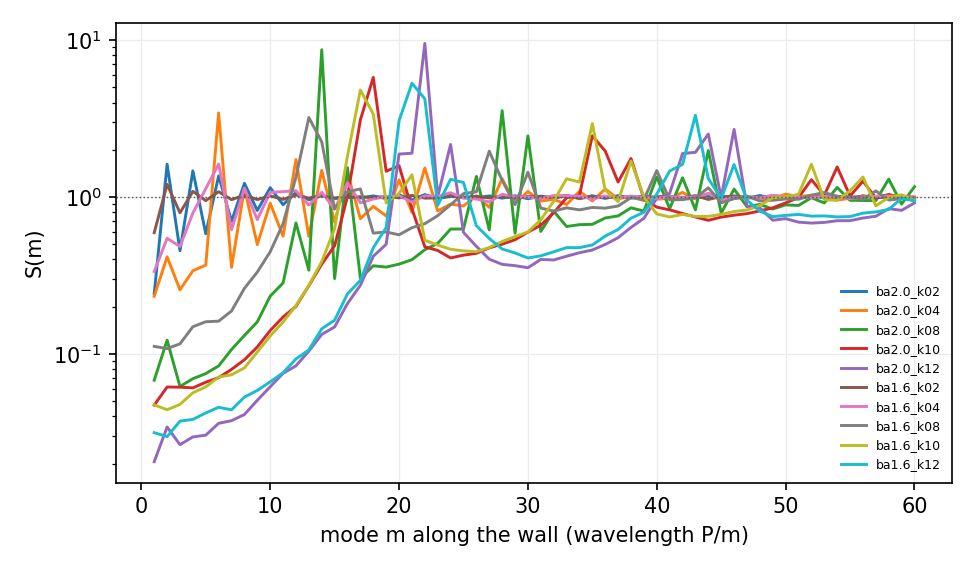
\includegraphics[width=0.7\textwidth]{wf_S_kscan.png}
\caption{$k$ scan (half-length $1.53\,\la$): the wall lattice reappears as $k$ grows.}\label{fig:wfk}
\end{figure}
\begin{figure}[H]\centering
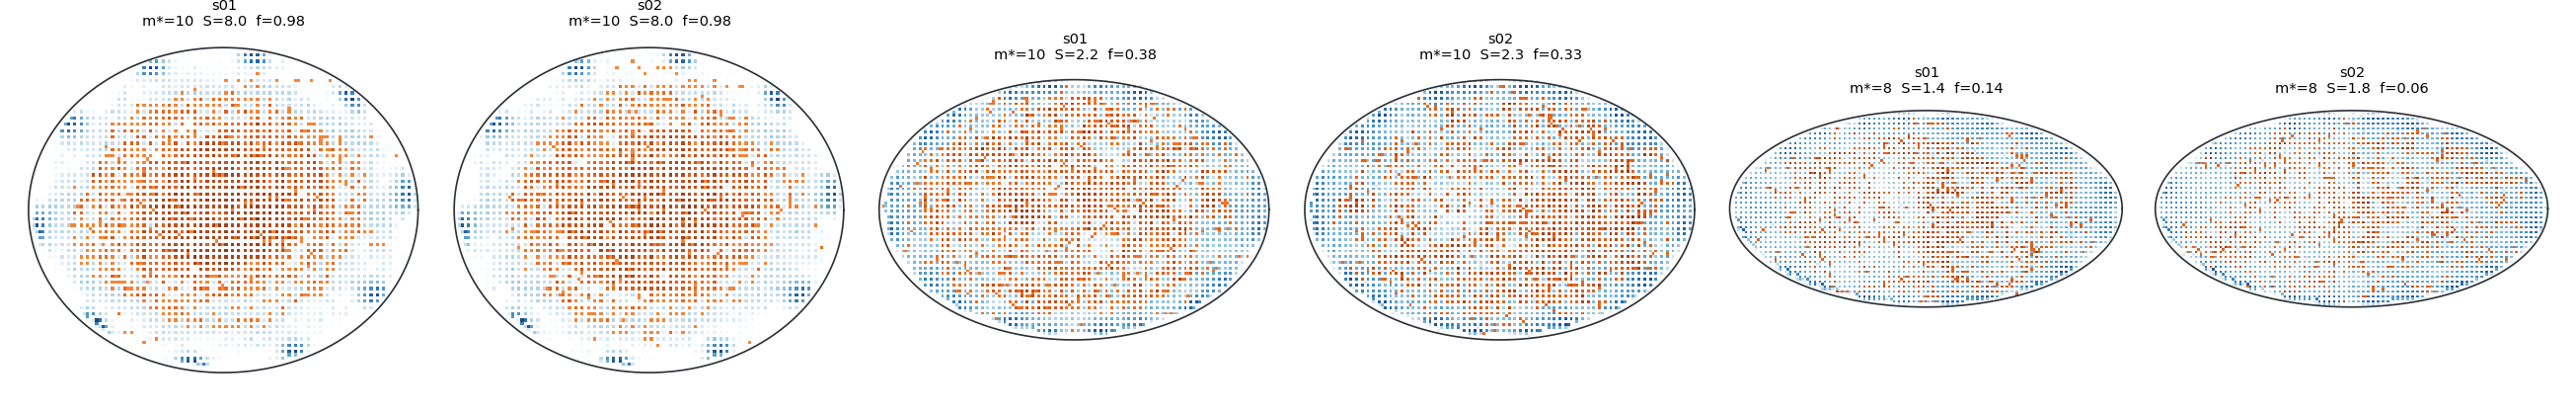
\includegraphics[width=\textwidth]{wf_maps_ellipses.png}\\[4pt]
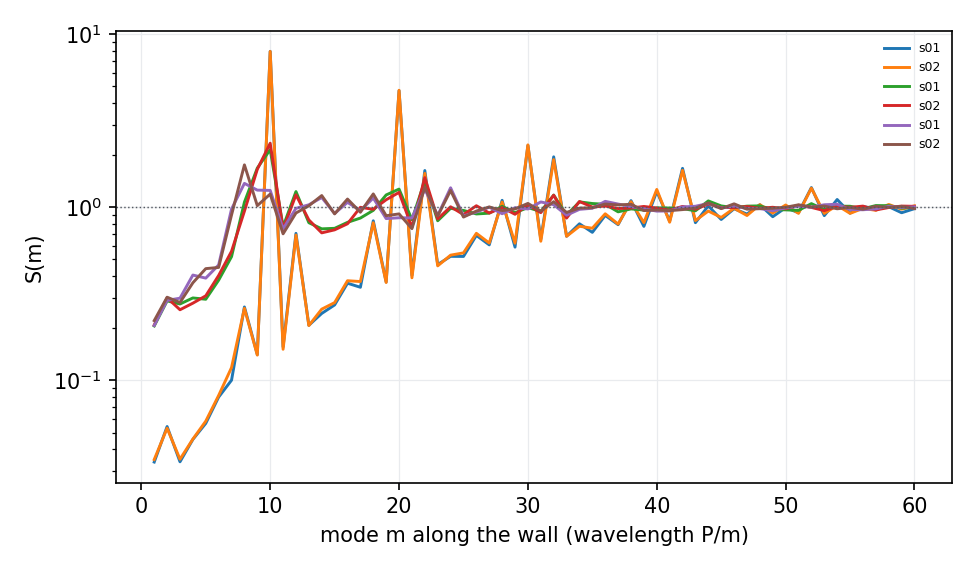
\includegraphics[width=0.7\textwidth]{wf_S_ellipses.png}
\caption{Ellipses: maps and $S(m)$.}\label{fig:wfell}
\end{figure}
\begin{figure}[H]\centering
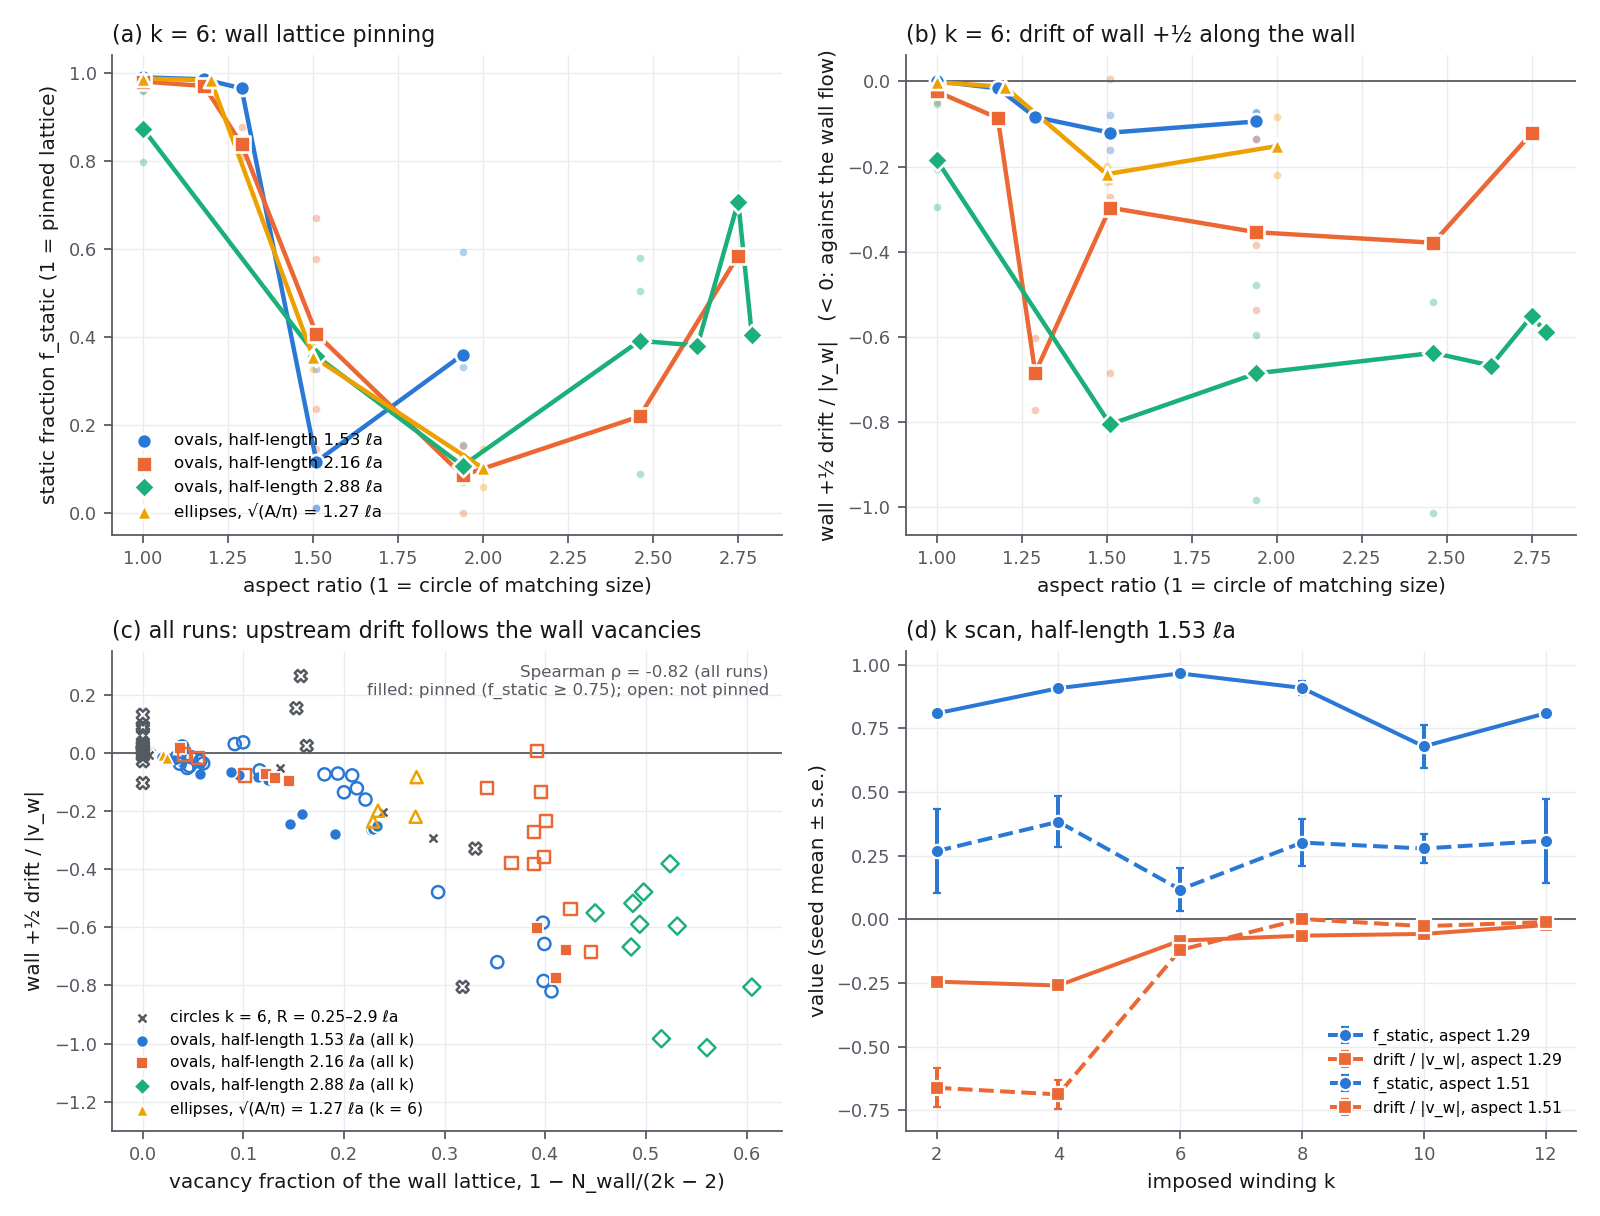
\includegraphics[width=\textwidth]{wall_dynamics.png}
\caption{\textbf{Wall lattice dynamics, ovals and ellipses against circles.} (a) Static fraction against aspect ratio ($k=6$; circles of
matching size at aspect 1, in the colour of the family they match: H34 $\leftrightarrow$ $1.43\,\la$, H48 $\leftrightarrow$ 2.15,
H64 $\leftrightarrow$ 2.87, ellipses $\leftrightarrow$ 1.23). (b) Per-defect drift of wall $+\half$ along the wall divided by the
near-wall flow speed $|v_w|$ (negative = upstream). (c) Drift against the vacancy fraction $1-N_\mathrm{wall}/(2k-2)$, all runs (filled:
pinned lattice, $f_\mathrm{static}\ge0.75$). (d) $k$ scan.}\label{fig:walldyn}
\end{figure}
\begin{itemize}
  \item \textbf{No sliding ordered layer in ovals either.} Where a lattice exists it is pinned (lattice phase speed $\approx0$). Where the
        order is weak ($S/N\lesssim0.4$) the phase of the lattice mode is noise, so the per-defect drift replaces it.
  \item \textbf{Pinning is lost with elongation} ($f_\mathrm{static}$ 0.97 $\to$ 0.1--0.4 from aspect 1.2 to 1.5), at the same aspect
        ratio as the charge split (Sec.~\ref{sec:scharge}); the H48 $b/a=2.0$ oval is the intermediate case: still pinned (0.81--0.88) but
        with only $\approx6$ of 10 sites occupied.
  \item \textbf{The near-wall flow turns with the bulk vortex} (sign agreement 100\% with one strong vortex; 60--90\% in elongated
        cavities, where $|v_w|$ drops from 0.2--0.35 to 0.03--0.07).
  \item \textbf{Wall $+\half$ creep against the wall flow, at a rate set by the vacancies of the lattice, not by its pinning:} Spearman
        $\rho_s=-0.82$ between drift$/|v_w|$ and the vacancy fraction over all runs ($-0.93$ among pinned lattices), against $+0.18$ for
        $f_\mathrm{static}$. Full circles: no drift. The H48 $b/a=2.0$ oval: pinned, 41\% empty, creeps at 69\% of the wall flow.
        Elongated ovals: $-10$ to $-80\%$. Reading: defects hop upstream into empty sites, so the vacancies travel downstream.
  \item \textbf{Crowded walls stop the creep:} in the $k$ scan it vanishes from $k=6$--8 on as the occupancy reaches 0.9--0.97;
        likewise in the pinched oval at $k=12$--20.
  \item Caveats: drift ratios are noisy for tiny circles without a vortex and for single-seed cavities; the drift includes defects
        entering or leaving the wall band. Circle drifts are normalised by the near-wall flow here; the circle sliding speeds in
        Sec.~\ref{sec:clattice} by the interior flow.
\end{itemize}

\subsection{Are the wall defects stationary, and where along the wall do they sit?}\label{sec:stationary}
Two direct tests of the protection of the wall layer (methods: Sec.~\ref{sec:m-tips}): how far a wall $+\half$ travels along the
wall while it stays in the wall band, and how the wall defects are distributed between the tips and the flanks of the ellipses.
\begin{table}[H]\centering\small
\caption{Along-wall travel of wall $+\half$ ($k=6$). For every pair of frames 50 or 500 time units apart in which a track stays within
4 cells of the wall throughout: number of pairs, median along-wall displacement $|\Delta s|$, and fraction with $|\Delta s|$ larger than
half the site spacing $P/(2(2k-2))\approx9$--10 cells (15 cells for the $2.15\,\la$ circle). The detection jitter is $\approx1$ cell.
Seed 1 unless two seeds are given (\texttt{reports/master/data/wall\_travel.txt}).}\label{tab:travel}
\begin{adjustbox}{max width=\textwidth}
\begin{tabular}{lcccccc}\toprule
& \multicolumn{3}{c}{lag 50} & \multicolumn{3}{c}{lag 500}\\
cavity & pairs & median $|\Delta s|$ & $>\frac12$ spacing & pairs & median $|\Delta s|$ & $>\frac12$ spacing\\\midrule
circle $1.43\,\la$ (2 seeds) & 37\,500 & 0.90--0.97 & 0--0.1\% & 23\,000 & 0.93 & 0--0.1\%\\
circle $2.15\,\la$ & 32\,779 & 1.15 & 0 & 9\,324 & 1.15 & 0\\
passive ellipses $\varepsilon=1.5$, 2.0 & 13\,700 & 0.99--1.00 & 0 & 8\,500--9\,300 & 1.05--1.22 & 0\\
ellipse $\varepsilon=1.2$ (2 seeds) & 35\,300 & 0.98--1.00 & 0--0.1\% & 18\,600--19\,500 & 0.97--0.98 & 0\\
oval $b/a=2.5$ (aspect 1.17) & 34\,925 & 0.97 & 0.1\% & 18\,072 & 0.97 & 1.4\%\\
ellipse $\varepsilon=1.5$ (2 seeds) & 18\,000 & 1.47--1.50 & 3.2--3.3\% & 607--923 & 2.0--3.1 & 24--31\%\\
ellipse $\varepsilon=2.0$ (2 seeds) & 16\,200--16\,600 & 1.95--2.00 & 3.1--3.6\% & 149--306 & 2.3--8.4 & 9--34\%\\
oval $b/a=1.6$ & 18\,820 & 1.48 & 3.7\% & 1\,165 & 2.06 & 20\%\\
oval $b/a=1.3$ & 21\,143 & 1.98 & 4.0\% & 1\,715 & 2.05 & 12\%\\\bottomrule
\end{tabular}
\end{adjustbox}
\end{table}
\begin{itemize}
  \item \textbf{Round cavities keep a protected, stationary layer.} In circles, the $\varepsilon=1.2$ ellipse and the $b/a=2.5$ oval the
        wall defects do not move beyond the detection jitter even over 500 time units, exactly as in the passive cavities, and
        30--70\% of the wall-band pairs at lag 50 are still in the band at lag 500 (28\% for the $2.15\,\la$ circle, 52--61\% for the other
        round cavities, 62--68\% passive).
  \item \textbf{In elongated cavities the wall defects wander and leave.} Within 50 time units they move twice as far along the wall
        ($1.5$--2 cells) and 3--4\% shift by more than half a site spacing; after 500 time units only 1--8\% are still in the wall band
        (the fast escape of Sec.~\ref{sec:ssurv}), and 9--34\% of those have shifted by more than half a spacing. The motion is
        individual wandering and hopping, not a sliding lattice (lattice phase speed $\approx0$), with a net upstream drift
        (Fig.~\ref{fig:walldyn}).
\end{itemize}
\begin{table}[H]\centering\small
\caption{Ellipses, $k=6$: spacing of the wall defects at the tips and on the flanks. Per frame, the arclength gaps between neighbouring wall
$+\half$ are assigned to the tips (gap midpoint at $|x|>A/\sqrt2$) or to the flanks; density ratio $=\langle\text{gap}\rangle_\text{flank}/
\langle\text{gap}\rangle_\text{tip}$: 1 for uniform spacing, $\varepsilon$ for the conductor distribution (the one that screens the interior
completely). Theory: passive equilibrium of 12 $+\half$ with uniform winding per arclength (Sec.~\ref{sec:theory}).
(\texttt{reports/master/data/wall\_gaps.txt})}\label{tab:tips}
\begin{adjustbox}{max width=\textwidth}
\begin{tabular}{lcccc}\toprule
ellipse (tip gap / flank gap in cells, density ratio) & passive simulation & active simulation (2 seeds) & passive theory & conductor\\\midrule
$\varepsilon=1.2$ & 15.1 / 14.7, \textbf{0.97} & 19.8 / 17.2, \textbf{0.87} & 14.8 / 14.9, 1.00 & 1.2\\
$\varepsilon=1.5$ & 15.5 / 15.1, \textbf{0.98} & 27.5 / 21.2, \textbf{0.77} & 15.2 / 15.3, 1.01 & 1.5\\
$\varepsilon=2.0$ & 16.3 / 16.1, \textbf{0.98} & 29.7 / 24.6, \textbf{0.83} & 16.1 / 16.1, 1.01 & 2.0\\\bottomrule
\end{tabular}
\end{adjustbox}
\end{table}
\begin{itemize}
  \item \textbf{Passive:} the imposed defects are evenly spaced along the arclength (density ratio 0.97--0.98), as the anchoring imposes and
        as the elastic theory predicts for winding uniform in arclength (1.00--1.01). They do not move towards the screening (conductor)
        distribution, which would need gaps $\varepsilon$ times smaller at the tips.
        \emph{Correction:} an earlier version compared the number of wall defects per unit length at the tips and on the flanks and read
        a tip excess growing with $\varepsilon$; with 12 discrete defects that count is set by how the ring sits (6 of 12 in the tip regions
        in every passive run) and does not measure the spacing.
  \item \textbf{Active:} the gaps at the tips are 15--30\% larger than on the flanks (density ratio 0.77--0.87): activity depletes the tips,
        away from the screening distribution. This holds even for $\varepsilon=1.2$, which keeps its layer, so tip depletion alone does not mean
        loss of the layer.
  \item \textbf{Reading.} The passive layer is uniform, so an ellipse is screened less well than a circle; the theory (Sec.~\ref{sec:theory})
        puts the leftover field in the inner part of the cavity at $\lesssim0.06\,\pi K$ for $\varepsilon=2$, small compared with the energies of
        approach near the wall. In the active ellipses the defects wander, deplete the tips, drift upstream and escape: the flow, not the
        weak unscreened elastic field, drives the loss of the layer. 1--2 seeds per shape; the running shape sweep will repeat both measures
        at all sizes and densities with 3 seeds.
\end{itemize}
